%!TEX root = ../thesis.tex

\chapter{Background}


% \section{Notation}

% The set of \(n \times m\) matrices with real-valued entries is denoted as \(\R^{n\times m}\).

% The norm symbol \(\norm{\cdot}\) without any additional qualifiers denotes the standard Euclidean norm for a vector, and the spectral (operator) norm induced by the Euclidean norm, i.e. for an \(n \times n\) matrix \(A\)
% \[
% 	\norm{A} = \sup\left\{\frac{\norm{Av}}{\norm{v}}\,\middle|\,v \in \R^n, \, \norm{v} \neq 0\right\}.
% \]


% For example, we say that a random variable \(A\) is equal to another random variable \(B\) almost surely (a.s.) if \(P\left(A = B\right) = 1\).




\section{Results from dynamical systems}

\begin{equation}
	\dod{w_t}{t} = u\left(w_t, t\right), \qquad w_0 = x \in \Omega,
	\label{eqn:det_ode}
\end{equation}
where \(u: \Omega \times[0,T] \to \R^n\) describes the velocity at a point in space and time.

In the mathematical treatment of Lagrangian dynamics, and in particular Lagrangian coherent structures \citep{BalasuriyaEtAl_2018_GeneralizedLagrangianCoherent}, trajectories solving \eqref{eqn:det_ode} are summarised by the flow map.
The flow map is an operator mapping

The flow map can be defined formally as follows.
\begin{definition}[Flow map]
	Suppose \(t_1, t_2 \in [0,T]\).
	The \textbf{flow map} \(F_{t_1}^{t_2}: \R^n \to \R^n\) from time \(t_1\) to \(t_2\) associated with \eqref{eqn:det_ode} is the unique solution to
	\begin{equation}
		\dpd{F_{t_1}^{\tau}(x)}{\tau} = u\left(F_{t_1}^\tau(x), \tau\right), \qquad F_{t_1}^{t_1}(x) = x,
		\label{eqn:flow_map_ode}
	\end{equation}
	solved up to time \(\tau = t_2\).
	Equivalently,
	\[
		F_{t_1}^{t_2}(x) = x + \int_{t_1}^{t_2}{u\left(F_{t_1}^\tau(x), \tau\right)\dif\tau}.
	\]
\end{definition}
The flow map satisfies the following properties, under ASSUMPTIONS? 
For any \(r, s, t \in [0,T]\) and points \(x,w \in \R^n\),
\begin{enumerate}
	\item \(F_{s}^{t}\) is invertible with inverse
		\[
			\left[F_{s}^{t}\right]^{-1}\left(w\right) = F_{t}^{s}\left(w\right).
		\]
	\item \(F_s^{t}\left(F_{r}^{s}(x)\right) = F_{r}^{t}\left(x\right)\) 
\end{enumerate}

The gradient of the flow map satisfies a useful property; the equation of variations.
\begin{theorem}
	Let \(F_{t_1}^{t}\) be the flow map corresponding to \eqref{eqn:det_ode}.
	Then, the spatial gradient \(\nabla F_{t_0}^t(x)\) satisfies the equation of variations
	\begin{equation}
		\dpd{\nabla F_{t_1}^{t}(x)}{t} = \nabla u\left(F_{t_1}^{t}(x), t\right) \nabla F_{t_1}^{t}(x).
		\label{eqn:eqn_of_variations}
	\end{equation}
\end{theorem}
\begin{proof}
	Taking the gradient on both sides of \eqref{eqn:flow_map_ode} and using the chain rule gives
	\[
		\nabla\left(\dpd{F_{t_1}^{t_2}(x)}{t}\right) = \nabla u\left(F_{t_1}^{t}(x), t\right) \nabla F_{t_1}^{t}(x).
	\]
	SMOOTHNESS
\end{proof}


% \subsection{Lagrangian coherent structures}
% \td{Briefly discuss LCSs. Do not need to go into too much detail here. Mention whatever is relevant}

An important inequality for establishing bounds 

\begin{theorem}[Gr\"onwall's inequality]\label{thm:gronwall}
	Let \(\alpha, \beta, u: [a,b] \to \R\) be functions such that \(\beta\) and \(u\) are continuous and that the negative part of \(\alpha\) is integrable on every closed and bounded subset of \([a,b]\).
	Then, if \(\beta\) is non-negative and for all \(t \in [a,b]\),
	\[
		u(t) \leq \alpha(t) + \int_a^t{\beta(\tau)u(\tau)\dif\tau}
	\]
	then
	\[
		u(t) \leq \alpha(t) + \int_a^t{\alpha(\tau)\beta(\tau)\exp\left(\int_\tau^{t}{\beta(s)\dif s}\right)\dif\tau}.
	\]
	Additionally, if \(\alpha\) is non-decreasing, then
	\[
		u(t) \leq \alpha(t) \exp\left(\int_a^t{\beta(\tau)\dif\tau}\right)
	\]
\end{theorem}

% \section{Results from probability theory}



% \subsection{The Dirac-delta distribution}


% The Dirac-delta probability measure has the property that for any measurable function \(f: \R^n \to \R^n\), 
% \[
% 	\int_{\R^n}{f\dif \delta[x_0]} = f(x_0)
% \]



\section{Stochastic differential equations}

For an introduction to stochastic differential equations, see \citet{Oksendal_2003_StochasticDifferentialEquations} or \citet{KallianpurSundar_2014_StochasticAnalysisDiffusion}.


\begin{definition}\label{def:wiener}
	The (one-dimensional) \emph{canonical Wiener process} is a stochastic process \(W_t\) taking values in \(\R\) and satisfying the following properties:
	\begin{romanate}
	\item \(W_0 = 0\), 
	\item for every \(s > 0\), the increments \(W_{s + t} - W_{s}\) for \(t \geq 0\) are independent of \(W_r\) for all \(r < s\),
	\item \(W_{s + t} - W_t \isGauss{0, s}\) for all \(s,t > 0\), and 
	\item \(W_t\) is continuous in \(t\) almost surely.
	\end{romanate}
\end{definition}
Remarkably, these properties \emph{uniquely} define the Wiener process, with the property that for any \(t > 0\), \(W_t \sim \mathcal{N}\left(0, t\right)\), a Gaussian distribution with mean zero and variance \(t\).




The differential form of an \(n\)-dimensional It\^o stochastic differential equation is
\begin{equation}
	\dif y_t = u\left(y_t, t\right)\dif t + \sigma\left(y_t, t\right)\dif W_t,
	\label{eqn:gen_sde}
\end{equation}
where the solution \(y_t\) is a stochastic process taking values in \(\R^n\), \(u: \R^n \times \R \to \R^n\) is the drift and \(\sigma: \R^n \times \R \to \R^{n\times n}\) is the diffusivity.
The driving process \(W_t\) is the canonical, \(n\)-dimensional Wiener process as defined in \Cref{def:wiener}.
For a (possibly random) initial condition \(y_0\), the solution \(y_t\) to \eqref{eqn:gen_sde} satisfies
\begin{equation}
	y_t = y_0 + \int_0^t{u\left(y_\tau, \tau\right)\dif\tau} + \int_0^t{\sigma\left(y_\tau, \tau\right)\dif W_\tau}.
	\label{eqn:gen_sde_int}
\end{equation}
In the most general case, the drift \(u\) and diffusivity \(\sigma\) are permitted to themselves be random functions \cite{KallianpurSundar_2014_StochasticAnalysisDiffusion}, but in this thesis we assume that both are deterministic.
There is an alternative formulation of a stochastic differential equation, known as the Stratonovich interpretation, which defines the stochastic integral in \eqref{eqn:gen_sde_int} in a way that arises natural from physical considerations. 
In this thesis, we only consider It\^o stochastic differential equations, but there is a conversion between the two interpretations that requires modifying the drift term \(u\) of the SDE. 

As with deterministic differential equations, we are interested in knowing precisely when solutions to \eqref{eqn:gen_sde} exist, and whether these solutions are unique.

A solution to the stochastic differential equation can be defined rigorously \cite{KallianpurSundar_2014_StochasticAnalysisDiffusion}.
\begin{definition}
	A stochastic process \(\set{y_t}_{t \in [0,T]}\) taking values in \(R^n\) is said to be a \emph{strong solution} of \eqref{eqn:gen_sde} with initial condition \(y_0 = \xi\) if the following holds:
	\begin{enumerate}
		\item For each \(t\),
		\item
		      \[
			      \int_0^T{\left(\norm{u\left(y_t, t\right)} + \norm{\sigma\left(y_t, t\right)}^2\right)\dif t} < \infty \alsu
		      \]

		\item For each \(t \in [0,T]\),
		      \[
			      y_t = \xi + \int_0^t{u\left(y_\tau, \tau\right)\dif\tau} + \int_0^t{\sigma\left(y_\tau, \tau\right)\dif W_\tau} \quad \text{a.s.}
		      \]
	\end{enumerate}
\end{definition}

Solutions are known as \emph{strongly unique} if, for any two strong solutions \(x_t\) and \(y_t\) to \eqref{eqn:gen_sde} defined on the same measure space,
\[
	P\left(x_t = y_t, \quad \forall t \in \left[0,T\right]\right) = 1
\]
That is, \(x_t\) and \(y_t\) are equal almost surely.

We can now state the requirements for \eqref{eqn:gen_sde} to have unique solutions.
\begin{theorem}[\citet{KallianpurSundar_2014_StochasticAnalysisDiffusion}]
	Let \(u_i\) be the \(i\)th component of \(u\) and \(\sigma_{ij}\) the \((i,j)\)th component of \(\sigma\), for \(i,j = 1,\hdots,n\).
	Suppose that for each \(i,j = 1,\hdots,n\),
	\begin{romanate}
		\item \(u_i\) is Borel-measurable, and
		\item \(\sigma_{ij}\) is Borel-measurable.
	\end{romanate}
	Suppose further that for all \(t \in [0,T]\) and \(x,y \in \R^n\), there is a positive constant \(K\) independent of \(t\) and \(x, y\) such that
	\begin{romanate}
		\setcounter{enumi}{2}
		\item \(\norm{u(x,t)}^2 + \norm{\sigma(x,t)}^2 \leq K\left(1 + \norm{x}^2\right)\) a.s.
		\item \(\norm{u\left(x,t\right) - u\left(y,t\right)}^2 + \norm{\sigma\left(x,t\right) - \sigma\left(y,t\right)}^2 \leq K\norm{x - y}\) a.s.
	\end{romanate}
	Then, \eqref{eqn:gen_sde} has a strongly unique strong solution.
\end{theorem}
\begin{proof}
	See Theorem 6.2.1 of \cite{KallianpurSundar_2014_StochasticAnalysisDiffusion}, for instance.
\end{proof}



\subsection{Analytical tools for It\^o calculus}
There are several tools available for the analytic treatment of It\^o integrals and solutions to stochastic differential equations, which we make use of throughout.
The first is It\^o's isometry, which relates the expectation of an It\^o integral to that of a deterministic one and is useful for computing moments. 
\begin{theorem}[It\^o's Isometry]\label{thm:ito_isom}
	Let \(f: \Omega \times [0,T] \to \R\) be an It\^o integrable stochastic process. 
	Then, for any \(t \in [0,T]\)
	\[
		\avg{\left(\int_0^t{f\left(\omega, \tau\right)\dif W_\tau}\right)^2} = \avg{\int_0^t{f\left(\omega, \tau\right)^2\dif\tau}}
	\]
\end{theorem}
\begin{proof}
	It\^o's isometry typically arises in the formal construction of the It\^o integral. 
	See ?? for instance.
\end{proof}

Next, we have It\^o's Lemma (or the It\^o Formula), which is a change-of-variables formula in stochastic calculus and can be thought of as a generalisation of the chain rule from deterministic calculus.
We state and use the multidimensional form of the Lemma for solutions to It\^o stochastic differential equations, although more general forms exist (e.g. see Theorem 5.4.1 of \cite{KallianpurSundar_2014_StochasticAnalysisDiffusion}).
\begin{theorem}[It\^o's Lemma]
	Let \(X_t\) be the strong solution to the stochastic differential equation
	\[
		\dif X_t = a\left(X_t, t\right)\dif t + b\left(X_t, t\right)\dif W_t,
	\]
	where \(a: \R^n \times [0,\infty) \to \R^n\), \(b: \R^n \times [0,\infty) \to \R^{n\times p}\) and \(W_t\) is the canonical \(p\)-dimensional Wiener process.
	If \(f: \R^n \times [0, \infty) \to \R^m\) is twice continuously-differentiable, then the stochastic process \(Y_t \coloneqq f\left(X_t, t\right)\) is a strong solution to the stochastic differential equation
	\begin{align*}
		\dif Y_t & = \left(\dpd{f}{t}\left(X_t, t\right) + \nabla f\left(X_t, t\right) a\left(X_t, t\right) + \frac12\mathrm{tr}\left[b\left(X_t, t\right)^{\T} \nabla\nabla f\left(X_t, t\right) b\left(X_t, t\right)\right] \right)\dif t \\
		         & \qquad\qquad\qquad\qquad + \nabla f\left(X_t, t\right)b\left(X_t, t\right) \dif W_t.
	\end{align*}
\end{theorem}
\begin{proof}

\end{proof}

Our third and final result is the Burkholder-Davis-Gundy inequality, which when applied to stochastic integrals provides bounds on the expected norm.
\begin{theorem}[Burkholder-Davis-Gundy Inequality]
	Let \(M_t\) be an It\^o-integrable stochastic process taking values in \(\R^n\).
	Then, for any \(p > 0\) there exists constants \(c_p, C_p > 0\) independent of the stochastic process \(M_t\) such that
	\[
		c_p\avg{\left(\int_0^t{\norm{M_\tau}^2\dif \tau}\right)^p} \leq \avg{\sup_{\tau \in \left[0, t\right]}\norm{\int_0^\tau{M_s\dif W_s}}^{2p}} \leq C_p\avg{\left(\int_0^t{\norm{M_\tau}^2\dif \tau}\right)^p}.
	\]
\end{theorem}
\begin{proof}

\end{proof}



\subsection{The Fokker-Planck equation}


The probability density function \(\rho: \R^n \times [0,T] \to [0,\infty)\) for the solution to \eqref{eqn:gen_sde} at time \(t \in [0,T]\) is the solution to the corresponding Fokker-Planck equation \cite{Risken_2012_FokkerPlanckEquationMethods}
\begin{equation}
	\dpd{\rho}{t} = \frac12\nabla\cdot\nabla\cdot\left(\rho\sigma\sigma^{\T}\right) - \nabla\cdot\left(\rho u\right)
	\label{eqn:fp_eqn}
\end{equation}	
subject to some initial density \(\rho\left(x,0\right)\) given by the initial condition to \eqref{eqn:gen_sde}.
For a fixed and deterministic initial condition \(y_0 = x\), the corresponding initial condition to \eqref{eqn:fp_eqn} is the Dirac-delta distribution centred at \(x\). 

For certain choices of the drift \(u\) and diffusivity \(\sigma\), \eqref{eqn:fp_eqn} reduces to several other well-known partial differential equations, including:
\begin{itemize}
	\item When \(\sigma \equiv D\), a scalar constant, then \eqref{eqn:fp_eqn} is the convection-diffusion equation with velocity field \(u\) and diffusivity \(D\).
\end{itemize}
\enlargethispage{3\baselineskip}
\begin{tikzpicture}
			\node (hold) at (0,0) {};
			\node[rotate=31.41592653587932384626433832795028841971693993751058209749445923078164062862089986280534211706798407] (poop) at (15,0) {\tiny poop}; 
		\end{tikzpicture}

	\begin{itemize}	\item When \(\sigma \equiv 0\), i.e. there is no diffusion, then \eqref{eqn:fp_eqn} is the continuity equation with velocity field \(u\).
\end{itemize}
The connection between the Fokker-Planck equation and the SDE \eqref{eqn:gen_sde} means that the solutions to each of these PDEs can be equivalently thought of as the time-evolution of the probability density of an SDE. 



% \section{Aspects of stochastic parameterisation}
% When using deterministic systems to model real-world phenomena, there are many ways in which uncertainty can arise.
% For instance,

% Stochastic parameterisation is a
% These unresolved subgrid effects are accounted for by introducing stochastic noise into the otherwise deterministic model.

% \citet{BernerEtAl_2017_StochasticParameterizationNew}

% \citet{LeutbecherEtAl_2017_StochasticRepresentationsModel}

% \subsection{Additive versus multiplicative noise}

% When \(\sigma = \sigma(t)\) depends only on \(t\), then noise is considered \emph{additive}.
% If there is spatial dependence in \(\sigma\), i.e. \(\sigma = \sigma(x,t)\), then the noise considered \emph{multiplicative}.



% For instance, \citet{SuraEtAl_2005_MultiplicativeNoiseNonGaussianity} shows that the non-Gaussian statistics observed in atmospheric regimes can arise from linear models with multiplicative noise.



\subsection{Some explicitly solvable SDEs}
In general, the solution to a stochastic differential equation cannot be expressed analytically, either as an explicit expression involving the Wiener process \(W_t\) or as a probability measure or density function. 
At best, most solutions can be written in terms of an It\^o integral which can otherwise not be simplified.
However, there are several simple examples for which a solution can be written, and even time-marginal probability density functions can be derived.
Here, we list several examples which are used to validate theory and test algorithms throughout this thesis.


\begin{example}[Ornstein-Uhlenbeck Process]

\end{example}

\begin{example}[Ben\^e's SDE]
	The \(1\)-dimensional stochastic differential equation 
	\begin{equation}
		\sde{x_t}{\tanh\left(x_t\right)}{},
		\label{eqn:bene_sde}
	\end{equation}
	is known as \emph{Ben\^e's stochastic differential equation} \cite{SarkkaSolin_2019_AppliedStochasticDifferential}.
	The probability density function of a weak solution of \eqref{eqn:bene_sde} can be derived using an appropriate change of measure with Girsanov's theorem. 
	A proof of this, and the derivation of a weak solution to \eqref{eqn:bene_sde} are provided in Section 7.3 of \cite{SarkkaSolin_2019_AppliedStochasticDifferential}.
	The probability density function \(p: \R \times \left(0,\infty\right) \to \left[0,\infty\right)\) for the solution \(x_t\) at time \(t > 0\) is given by 
	\begin{equation}\label{eqn:bene_sde_pdf}
	p(x,t) = \frac{1}{\sqrt{2\pi t}}\frac{\cosh\left(x\right)}{\cosh\left(x_0\right)}\exp\left[-\frac{t}{2} - \frac{1}{2t}\left(x - x_0\right)^2\right],
\end{equation}
	where \(x_0 \in \R\) is a fixed initial condition.
	This probability density function is plotted, for the initial condition \(x_0 = 1/2\) and various times, in \Cref{fig:bene_pdf}.
	The resulting density is not symmetric and bimodal, with the two modes moving apart in the positive and negative \(x\)-directions respectively as \(t\) increases.
	For fixed \(t\), the probability density function can be expressed as the mixture of two Gaussians with respective means \(x_0 + t\) and \(x_0 - t\), with details provided in \Cref{app:bene_calculations}.
	This expression allows easy calculation of the mean and expectation of \(x_t\), as 
	\[
		\avg{x_t} = \frac{1}{2\cosh\left(x_0\right)}\exp\left(-\frac{t}{2}\right)\left(\left(x_0 + t\right)\exp\left[\frac{t}{2} +x_0\right] + (x_0 - t)\exp\left[\frac{t}{2} - x_0\right]\right).
	\]
	and 
	\[
		\var{x_t} = \mathbb{V}, \mathds{Z} \,  \mathbb{Z}, \R, \mathds{R}, \mathbb{C}, \mathbb{Q}, \mathbb{N}, \C, \Q, \N, \mathbf{R}, \bm{R}, \mathbf{N}, \bm{N}, \mathcal{R}, \mathfrak{R}, \mathds{1}
	\]
\end{example}
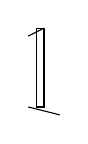
\begin{tikzpicture}
	\draw (0,0) -- (0,1) -- (0.1,1) -- (0.1,0) -- (0,0);
	\draw (-0.1,0.9) -- (0.1,1);
	\draw (-0.1,0) -- (0.3,-0.1);
\end{tikzpicture} $= \{0 \to 1\}$ 
% $$\left\{x \in \mathbb{R} \,\middle|\, x = \frac{1}{2}\right\} \left\{x \in \mathbb{R} \makebox[\widthof{\mid}]{\middle|} x = \frac{1}{2}\right\}$$

First \makebox[\widthof{some long text}]{poop} is always the best. :)

\newcommand{\plotbenepdf}[2]{
\begin{tikzpicture}\begin{axis}[
		ymin=0.0,
		xmin=-10.0,
		xmax=10.0,
		axis lines=center,
		axis on top=true,
		domain=-10:10,
		ylabel=$p$,
		xlabel=$x$,
		ytick=\empty,
		yticklabels={},
	]
	\addplot [mark=none,draw=black,thick,samples=500] {cosh(\x)*exp(-#2/2-1/(2 * #2)*(\x-#1)^2)/((2 * pi * #2)^(1/2) * cosh(#1))};
\end{axis}
\end{tikzpicture}
}

\begin{figure}
	\begin{center}
\begin{subfigure}{0.49\textwidth}
\plotbenepdf{1/2}{1}
	\caption{\(t = 1\)}
	\label{fig:bene_1}
\end{subfigure}
\begin{subfigure}{0.49\textwidth}
\plotbenepdf{1/2}{2.5}
	\caption{\(t = 2.5\)}
	\label{fig:bene_2.5}
\end{subfigure}
\begin{subfigure}{0.49\textwidth}
\plotbenepdf{1/2}{5}
	\caption{\(t = 5\)}
	\label{fig:bene_5}
\end{subfigure}
\begin{subfigure}{0.49\textwidth}
\plotbenepdf{1/2}{7.5}
	\caption{\(t = 7.5\)}
	\label{fig:bene_7.5}
\end{subfigure}
	\end{center}
	\caption{The probability density function \eqref{eqn:bene_sde_pdf} for the time-marginal solution of Ben\^e's SDE \eqref{eqn:bene_sde}, for the initial condition \(x_0 = 1/2\) at various times.
	The density function consists of two distinct modes that move further apart as \(t\) increases.}
	\label{fig:bene_pdf}
\end{figure}


%\section{Stochastic sensitivity}
\section{Poop sensitivity}

Following the nomenclature of fluid dynamics, given unsteady Eulerian velocity data \(u: \R^2 \times [0,T] \to \R^2\), the evolution of Lagrangian trajectories is governed by the ordinary differential equation 
\[
	\dod{x_t}{t} = u\left(x_t, t\right).
\]
Solutions can be summarised by the flow map \(F_{t_1}^{t_2}\), as in \Cref{def:flow_map}.
In most practical situations, the Eulerian velocity data driving ocean and atmospheric models relies upon measurements of estimates obtained on a low resolution spatial discretisation.
\citet{Balasuriya_2020_StochasticSensitivityComputable} introduces stochastic sensitivity as a new tool for directly quantifying the impact of Eulerian uncertainty on Lagrangian trajectories.
The evolution of Lagrangian trajectories is modelled as solution to a It\^o stochastic ordinary differential equation.

To directly account for these unresolved sources of uncertainty, the ``true'' Lagrangian trajectories evolve as solution to the stochastic differential equation
\begin{equation}
	\sde{y_t}{u\left(y_t, t\right)}{\epsilon\sigma\left(y_t, t\right)},
	\label{eqn:ss_sde},
\end{equation}
where \(0 < \epsilon \ll 1\) is a parameter quantifying the scale of the noise, \(\sigma:	\R^2\times[0,T] \to \R^{2\times 2}\) is the \(2\times 2\) diffusion matrix, and \(W_t\) is the canonical two-dimensional Wiener process.
In the original formulation \cite{Balasuriya_2020_StochasticSensitivityComputable}, \(\epsilon\) is a dimensionless parameter and \(\sigma\) is dimensional, but an alternative scaling technique relates \(\epsilon\) to spatial and velocity uncertainty scales in the data (see the follow-up work \cite{BadzaEtAl_2023_HowSensitiveAre,Balasuriya_2020_UncertaintyFinitetimeLyapunov,FangEtAl_2020_DisentanglingResolutionPrecision})
Since \(\sigma\) can vary by both space and time, the noise is multiplicative.
The diffusion matrix \(\sigma\) is specified \emph{a priori}, based on any knowledge of how uncertainty varies with space and time, e.g. from experimental considerations, observation error estimates.
If no such prior information is known, then \(\sigma \equiv I\), the \(2 \times 2\) identity matrix is the default choice.

To quantify uncertainty in a way that is independent of the noise scale \(\epsilon\), \citet{Balasuriya_2020_StochasticSensitivityComputable} defined the random variable \(z_\epsilon\left(x,t\right)\) on \(\R^2 \times [0,T]\) as
\[
	z_\epsilon\left(x,t\right) \coloneqq \frac{y_t - F_0^t(x)}{\epsilon}.
\]
The main aim is to compute statistics of \(z_\epsilon\) at the final time \(T\), so that of \(z_\epsilon\left(x,T\right)\).
\citet{Balasuriya_2020_StochasticSensitivityComputable} then considers the signed projection of \(z_\epsilon\left(x,T\right)\) onto a ray emanating from the deterministic position \(F_0^T(x)\) in a given direction, defining
\[
	P_\epsilon\left(x,\theta\right) \coloneqq \hat{n}^{\T} z_\epsilon(x,T),
\]
where \(\theta \in \left[-\pi/2, \pi/2\right)\) and
\[
	\hat{n}(\theta) = \begin{bmatrix}
		\cos{\theta} \\
		\sin{\theta}
	\end{bmatrix}.
\]
% \Cref{fig:sb_ss} is a pictorial representation of these quantities, with those associated with the deterministic equation \eqref{eqn:ode_det} in black and those with the stochastic equation \eqref{eqn:ss_sde} in blue.

% \begin{figure}
% 	\begin{center}
% 		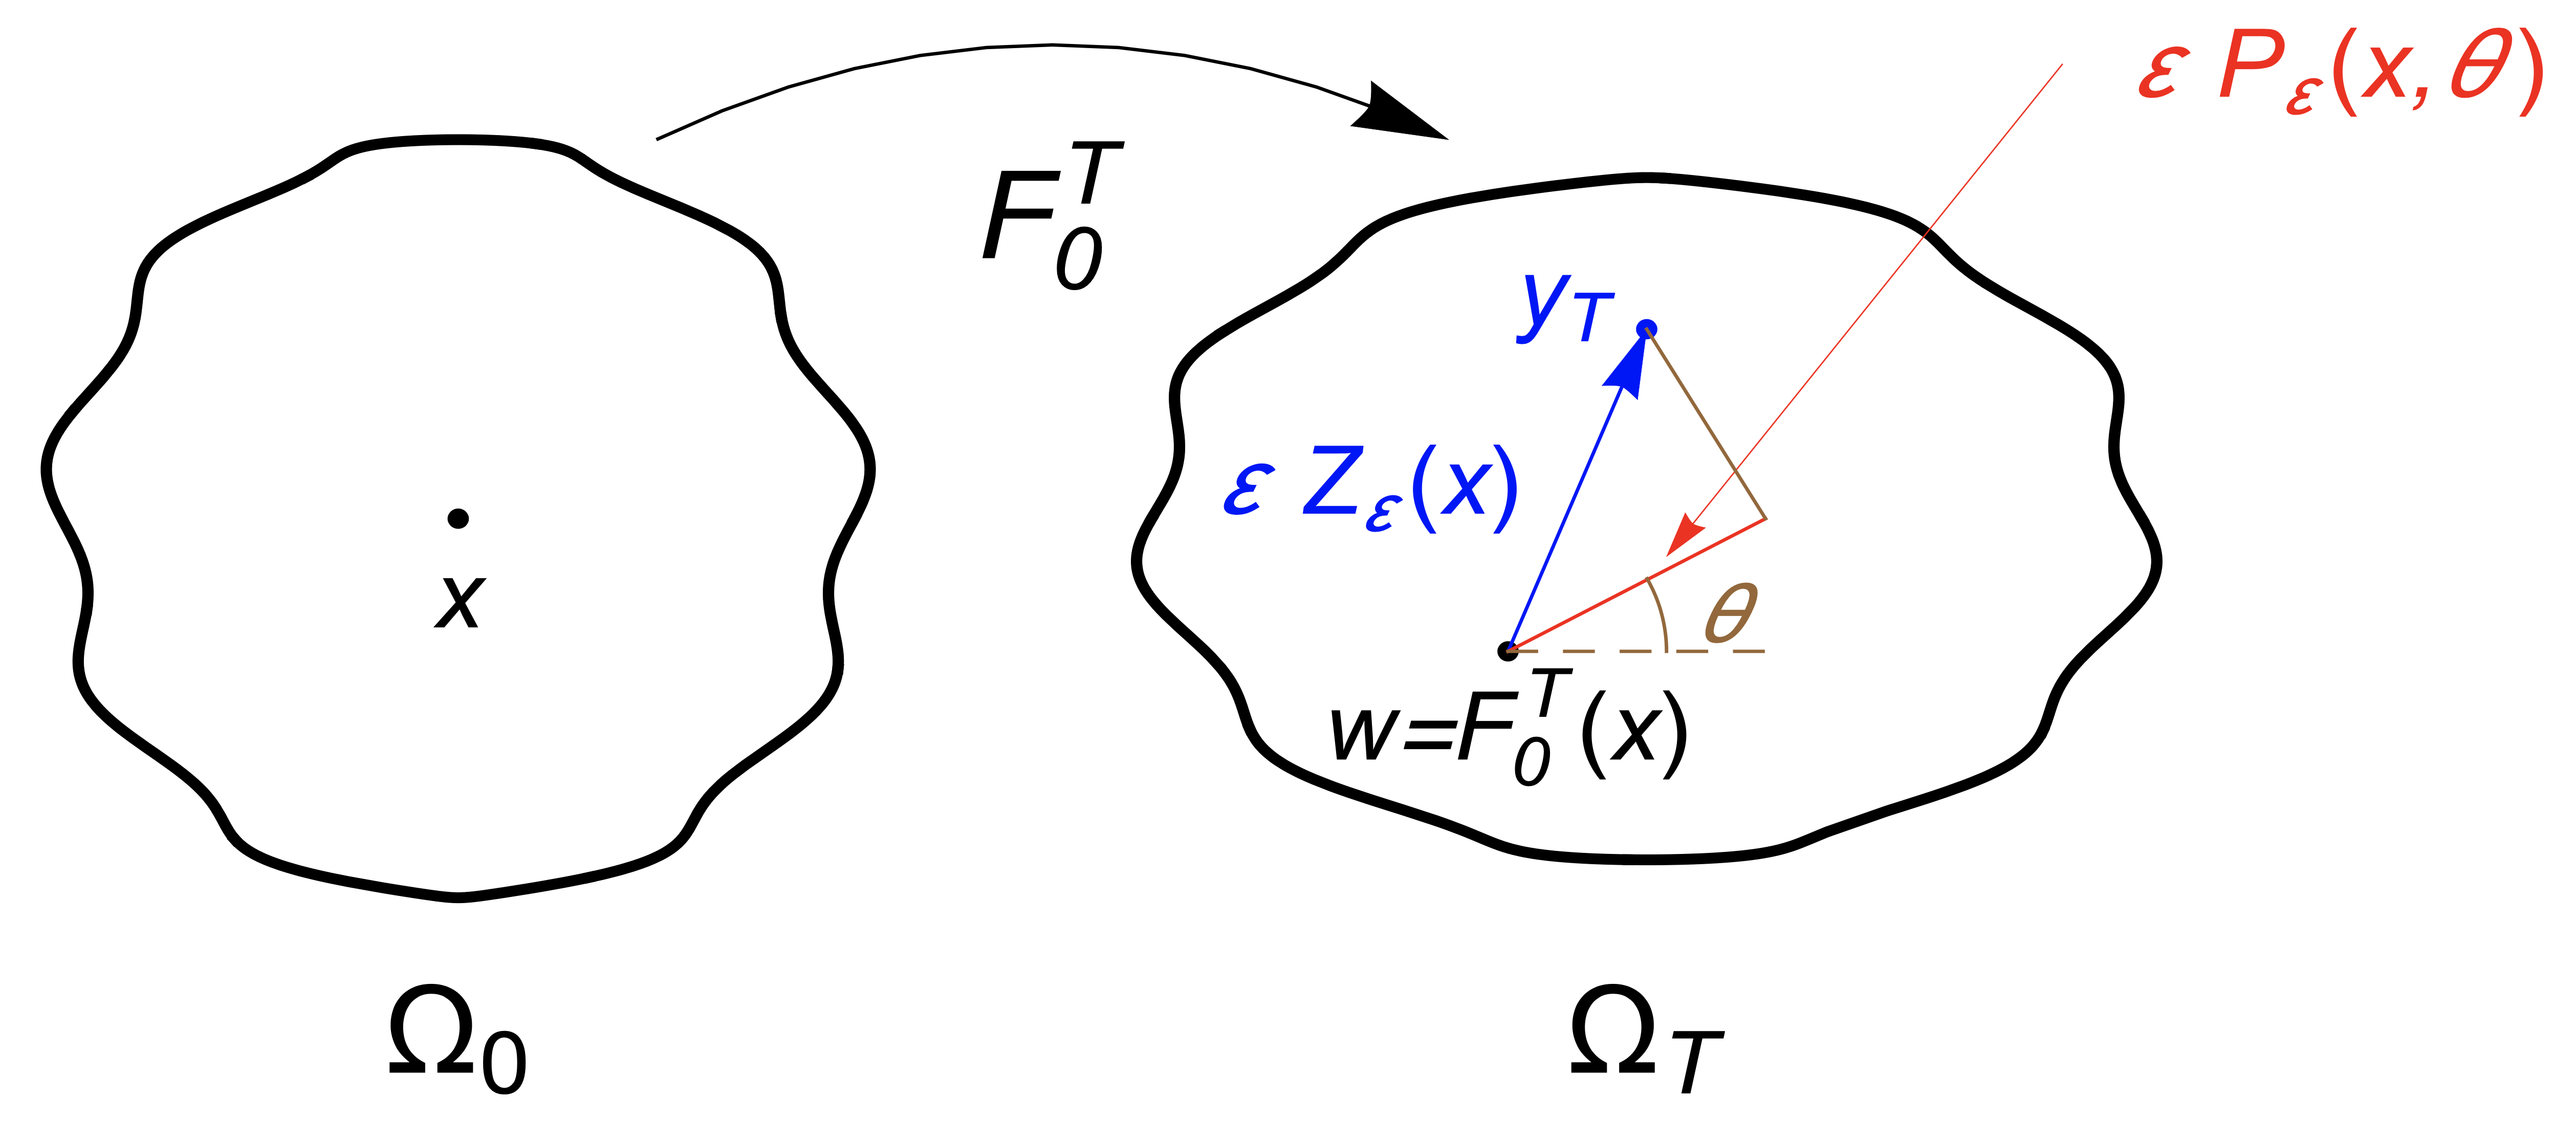
\includegraphics[width=\textwidth]{figures/sb_ss_diagram.png}
% 		\td{Might not actually have permission to reproduce this figure - SIAM would own it, right? I can just recreate it anyways.}
% 		\caption{.
% 		This is Figure 2.1. of \cite{Balasuriya_2020_StochasticSensitivityComputable}.}
% 		\label{fig:sb_ss}
% 	\end{center}
% \end{figure}


The statistics of \(z_\epsilon\left(x,T\right)\) and \(P_\epsilon(x,\theta)\) are considered in the limit as \(\epsilon\downarrow 0\), which provides a characterisation of the uncertainty of the model \emph{independently} of the scale of the noise.
\citet{Balasuriya_2020_StochasticSensitivityComputable} provided computable expressions for the mean and variance of \(P_\epsilon\left(x,\theta\right)\) in this limit of small noise, which we summarise here.
For proofs of these results, see the appendices of \cite{Balasuriya_2020_StochasticSensitivityComputable}.

The first result established by \citet{Balasuriya_2020_StochasticSensitivityComputable} is that the expected location is deterministic, in the following sense.
\begin{theorem}[\cite{Balasuriya_2020_StochasticSensitivityComputable}]
	For all \(x \in \R^2\),
	\[
		\lim_{\epsilon\downarrow 0}\avg{z_\epsilon(x,T)} = 0.
	\]
\end{theorem}

The variance of \(P_\epsilon\left(x,\theta\right)\) is used to assign a computable scalar measure of uncertainty to the trajectory.

\begin{definition}[\cite{Balasuriya_2020_StochasticSensitivityComputable}]
	\begin{alpharate}
		\item The \textbf{anisotropic uncertainty} is a scalar field \(A: \R^2\times\left[-\pi/2, \pi/2\right) \to [0,\infty)\) defined by
		\[
			A(x,\theta) \coloneqq \sqrt{\lim_{\epsilon\downarrow 0}\var{P_\epsilon(x,\theta)}}.
		\]

		\item The \textbf{stochastic sensitivity} is a scalar field \(S: \R^2 \to [0,\infty)\) defined by
		\[
			S^2(x) \coloneqq \lim_{\epsilon\downarrow 0}\sup_{\theta}{\var{P_\epsilon(x,\theta)}}.
		\]
	\end{alpharate}
\end{definition}

By employing techniques from both deterministic and stochastic calculus (i.e. Gr\"onwall's inequality, the Burkholder-Davis-Gundy inequality, It\^o's Lemma), Balasuriya further established expressions for both the anisotropic uncertainty and the stochastic sensitivity that are computable given only the flow map and velocity data.

\begin{theorem}[\cite{Balasuriya_2020_StochasticSensitivityComputable}]\label{thm:orig_s2_calculation}
	For \(x \in \R^2\), set \(w \coloneqq F_0^t(x)\).
	Then, for any \(\theta \in \left[-\pi/2, \pi/2\right)\),
	\[
		A(x,\theta) = \left(\int_0^T{\norm{\Lambda\left(x, t, T\right)J\hat{n}(\theta)}\dif t}\right)^{1/2},
	\]
	where
	\[
		\Lambda\left(x,t,T\right) \coloneqq e^{\int_t^T{\left[\nabla \cdot u\right]\left(F_0^\xi(x), \xi\right)\dif\xi}}\sigma\left(F_0^t(x), t\right)^{\T}J \nabla_w F_T^t\left(w\right),
	\]
	with the gradients \(\nabla_w\) of the flow map taken with respect to the mapped position \(w\), and
	\[
		J \coloneqq \begin{bmatrix}
			0 & -1 \\
			1 & 0
		\end{bmatrix}
	\]
	Additionally, stochastic sensitivity is computed as
	\[
		S^2(x) = P(x) + N(x),
	\]
	with
	\begin{align*}
		L(x) & \coloneqq \frac12\sum_{i=1}^2\int_0^T\left[\Lambda_{i2}\left(x,t, T\right)^2 - \Lambda_{i1}\left(x,t,T\right)^2\right]\dif t \\
		M(x) & \coloneqq \sum_{i=1}^2\int_0^T{\Lambda_{i1}\left(x,t,T\right)\Lambda_{i2}\left(x,t,T\right)\dif t}                           \\
		N(x) & \coloneqq \sqrt{L^2(x) + M^2(x)}                                                                                             \\
		P(x) & \coloneqq \abs{\frac12\sum_{i=1}^2\sum_{j=1}^2{\int_0^T{\Lambda_{ij}\left(x,t,T\right)^2\dif t}}},
	\end{align*}
	where \(\Lambda_{ij}\) is the \((i,j)\)-element of \(\Lambda\).
\end{theorem}








\subsection{Current applications \& shortcomings}
Since stochastic sensitivity is only a recent development, it has only been applied in a limited number of places so far.
Here, we briefly review the literature in which the original formulation stochastic sensitivity by \cite{Balasuriya_2020_StochasticSensitivityComputable} has been applied.

\begin{itemize}
	\item \citet{Balasuriya_2020_UncertaintyFinitetimeLyapunov} uses stochastic sensitivity to compute an error bound for the finite-time Lyapunov computation.


	\item \citet{FangEtAl_2020_DisentanglingResolutionPrecision} 


	\item \citet{BadzaEtAl_2023_HowSensitiveAre} investigate the impact of velocity uncertainty on Lagrangian coherent structures (e.g. see the reviews by \citet{BalasuriyaEtAl_2018_GeneralizedLagrangianCoherent} and \citet{HadjighasemEtAl_2017_CriticalComparisonLagrangian}) extracted as robust sets with stochastic sensitivity.
		The stochastic model \eqref{eqn:ss_sde} is used to generate realisations of Lagrangian trajectories subject to noise on the velocity field. 
		By directly capturing such uncertainty as a means of coherent set \citet{BadzaEtAl_2023_HowSensitiveAre} showed that robust sets extracted with stochastic sensitivity do SOMETHING.

\end{itemize}
There are several limitations to the work as presented in \cite{Balasuriya_2020_StochasticSensitivityComputable},
\begin{enumerate}
	\item The tools are restricted to two-dimensional models, and the constructions using projections have no obvious extension to \(n\)-dimensions.
	      Extending stochastic sensitivity to \(n\)-dimensions will enable application to a much broader class of models beyond the fluid flow context, including high-dimensional climate models.

	\item \citet{Balasuriya_2020_StochasticSensitivityComputable} only computes the expectation and variance of the projections \(P_\epsilon(x,\theta)\), which does not give us the distribution under the limit as \(\epsilon\) approaches 0.

	\item The computational formula for the anisotropic uncertainty and stochastic sensitivity, as described in \Cref{thm:orig_s2_calculation}, require knowledge of the divergence \(\nabla\cdot u\) of the velocity field, and computation of four integrals.
\end{enumerate}

An alternative approach to uncertainty quantification in Lagrangian dynamics was recently introduced by \citet{BranickiUda_2023_PathBasedDivergenceRates}, extending results from their earlier work in \cite{BranickiUda_2021_LagrangianUncertaintyQuantification}. 
However, the divergence approach does not provide any insight into the underlying probability distribution.
Moreover, stochastic sensitivity 


% \section{Gaussian mixture models}
% In this section, we briefly discuss Gaussian mixture models (GMMs), as a means of approximating highly non-Gaussian distributions in a computationally and analytically convenient manner.


